\chapter{Literature Review}
% Approximately 5000 words  

%%%%%%%%%%%%%%%
% Basic Layout
%%%%%%%%%%%%%%%
% Introduction to Road Safety research in Ireland - What is the extent of the methods we research driver behaviour % 500
% Introduction to Decision Neuroscience % 2000
    % Typical Tasks
    % DDM
    % The speed accuracy trade off
    % The Kelly lab
    % EMG - How to use EMG for predictive modelling/prepratory signals
% Introduction to Traffic & Driver behaviour research
    % Try make this one 2000

%%%%%%%%%%%%%%%
% Introduction to Road Safety in Ireland
%%%%%%%%%%%%%%%
% Want this to be ~1000 words in sections
% The main focus is: How do we research driver behaviour
\section{Road Safety in Ireland}
The study of road safety design, policy and research cannot be divorced from the context of its history and evolution. As large scale and long lasting pieces of infrastructure roads are inevitably a product of the time in which they were constructed. Therefore, as design standards and attitudes changed over time, so too did the perception and understanding of safety for different road users.

% Vehicular cycling and the insistence on behaviour of drivers and cyclist
\subsection{The Evolution of the Purpose of Roads}
Ireland has a long history of cycling based transportation dating from the invention of the first pedal-driven bicycle in 1840 until the present day. However, similar to most western nations, the invention and popularisation of the automobile caused revolutionary change in the design of roads. Streets which had long been dominated by people, trams, coaches and cyclists became exclusively reserved for the movement of the automobile \citep{southworthStreetsShapingTowns2013}. This involved the redesign of many urban streets and the rollout of a vast national road and motorway system, the largest infrastructural investment in Irish history \citep{obrienDrivingForce102019}. This re-prioritisation can be seen reflected in decades of road design standards and manuals  where little mention was made of the faciliation of safe cycling \citep{dotDesignManualUrban2013}.

\subsection{The Road Safety Authority \& Current Safety Policy}
Currently there are several governmental agencies and non-governmental agencies in Ireland who's remits involve the promotion and facilitation of safety on the roads. Of primary interest to this examination and cycling safety more generally are the Department of Transport (DOT), local councils and the Road Safety Authority (RSA) \citep{rsaRoadSafetyIreland2022}.

Local councils are responsible for the design, construction and maintenance of non-national roads. The DOT creates and updates road design manuals for the use of the councils. Their decisions are influenced by the data gathered and provided by the RSA who are further responsible for both public information and campaigning for best practice regarding road safety \citep{RoadSafetyReport2021}. While the policy of the DOT \& councils have changed in recent years in response to the urban planning infrastructural-based consensus on road safety, the RSA has continued to take an approach based on education and behavioural change of drivers \& cyclists \citep{rsaCyclistsCampaignRoad2022}.

\section{Driver Behaviour Research}
Recent efforts to study the decision making in driving scenarios has been dedicated to the improvement of self-driving algorithms. These models however have been focused on allowing automated vehicles to predict the behaviour of humans, but not on the underlying mechanics behind that human behaviour. Thus, it is the interaction between drivers and automated systems that is of concern, not necessarily the actual decision making of the drivers \citep{jiHierarchicalGametheoreticDecisionmaking2023, HeuristicsOrientedOvertaking}.

In the context of an overtaking decision, there have been a number of studies trying to quantify and predict behaviour. In \citet{stefanssonModelingDecisionmakingHuman2020}, a driving simulation study, a Kalman filter formulation was used to derive methods of mathematically predicting overtaking behaviour. In \citet{grayPerceptualProcessesUsed2005} the perceptual processes of drivers were examined with regard to oncoming cars in a driving simulator. It was found that some drivers will take risk well in access of acceptable levels due to inaccurate information and decision criteria.

Thus far, decision neuroscience techniques, the basis that this project is to be built on, have not been widely applied to driver decision making processes.

\section{Decision Neuroscience}
Decision Neuroscience (DN) as a field evolved from other decision study, distinguishing itself through the use of mathematical models to examine the underlying processes which result in a decision being made. These models can take many forms, a common framework being the drift diffusion model (DDM) developed by Ratcliff nearly 50 years ago to "deal with all aspects of the data in each paradigm [of decision making] (accuracy, response latency, and latency distributions)" \citep{ratcliffTheoryMemoryRetrieval1978}. It is a unifying model which can represent the results of a wide variety of different task and decision paradigms. It has also proven to be endlessly adaptable, with the changing of some crucial parameters allowing the fitting of complex situations with remarkable accuracy. 

\subsection{Speed-Accuracy Tradeoff}
In making a choice between one of two objects one faces a dilemma known as the speed-accuracy tradeoff (SAT). This process is an inverse relationship between the speed at which a decision is made and how accurate that decision will be \citep{spieserDecisionMotorContribution2017,bogaczNeuralBasisSpeed2010}. This tradeoff arises from the limited resources that an individual has on hand when faced with a decision which requires a rapid response. Should they wait for further information to ensure accuracy or is there simply insufficient time to do so? Quicker decisions are by nature less accurate as they allow for significantly less time for evidence accumulation. This phenomenon has been studied extensively in the abstract through the application of the mathematical modelling tools of DN. In the more recent times however, the neurological basis of it has also been examined in an attempt to not just predict, but also understand the physiological mechanisms behind decisions \citep{goldNeuralBasisDecision2007a,heitzNeuralMechanismsSpeedAccuracy2012}.

\subsection{The Drift Diffusion Model}
% Talk about the model in abstract
The DDM is a basic model of human decision making that can be used to understand decisions which correspond to the two alternative forced choice (2AFC) paradigm, where participants must make a binary decision quickly (within 2 seconds) with stimuli that are uncertain \citep{ratcliffDiffusionDecisionModel2008, myersPracticalIntroductionUsing2022}. The model allows an analogous understanding of the neurological mechanisms which cause a decision to be made. In DDM the two alternatives of the 2AFC decision are modelled as the upper and lower boundary of the decision space. Within this space, following the onset of a stimulus, evidence accumulates noisily to one of the two boundaries with an average slope modelled by the drift rate $\nu$. Once one of the two boundaries have been crossed the decision will be recorded as having occurred at that time. This gives rise to the characteristic right skewed reaction time distributions seen in typical decision tasks \citep{ratcliffTheoryMemoryRetrieval1978}. A schematic of this process can be seen in \ref{fig:DDM plot}.
\begin{figure}[H]
    \centering
    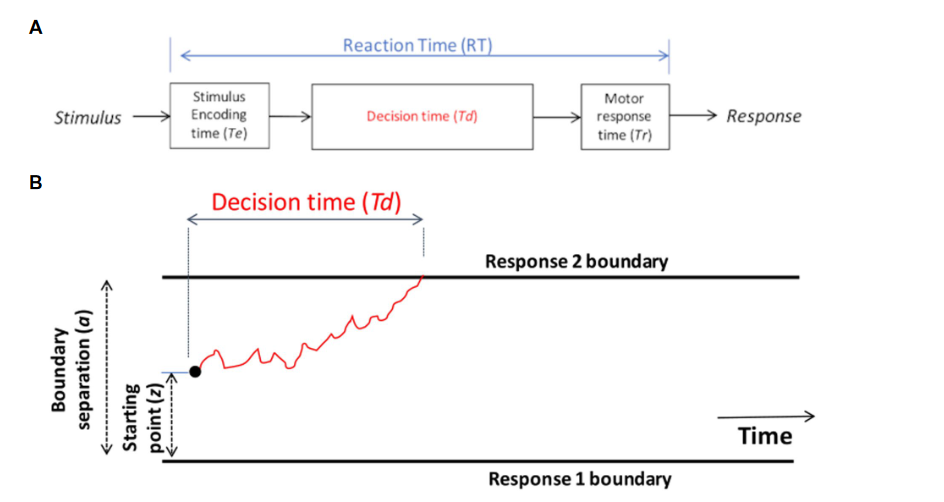
\includegraphics[width=0.75\linewidth]{figures/DDM.PNG}
    \caption{Schematic of the drift diffusion model (DDM). (A) Total reaction time to make a decision is composed of fixed stimulus encoding time $T_{e}$, decision time $T_{d}$ and motor response time $T_{r}$ (B) The noisy accumulation of data can be seen here from a starting point $z$ towards the two boundaries. The separation between the boundaries, seen here as $a$, can be manipulated with $z$ to bias the model towards one of the responses \citep{myersPracticalIntroductionUsing2022}}
    \label{fig:DDM plot}
\end{figure}

% random dot motion task
This model has been studied in detail using simple decision tasks such as the random dot motion (RDM) task, but has also been applied to more complicated tasks including the prediction of the detection of military target positioning \citep{heitzNeuralMechanismsSpeedAccuracy2012}. The RDM task is one of the most common in use in the field and has been altered for study in a variety of ways to examine different factors. The basic structure of the task is the discrimination between coherent and incoherent motion; the dots begin by moving incoherently and at the onset of the simulus a certain subset of the dots begin moving coherently in a direction \citep{brittenAnalysisVisualMotion1992}. The participant must respond when they have identified the presence of this stimulus. This task has been used to examine the effects of sleep deprivation, depression and, to help identify decision-related signals in the brain, among other applications \citep{ratcliffDiffusionModelOnechoice2011, kellyInternalExternalInfluences2013, whiteUsingDiffusionModels2010}. The task is useful in part because of the control it gives researchers over the difficulty of the task, forcing participants to make mistakes and giving a temporal distribution of both correct and incorrect reactions to fit models to.
% Another figure in here.
\begin{figure}[H]
    \centering
    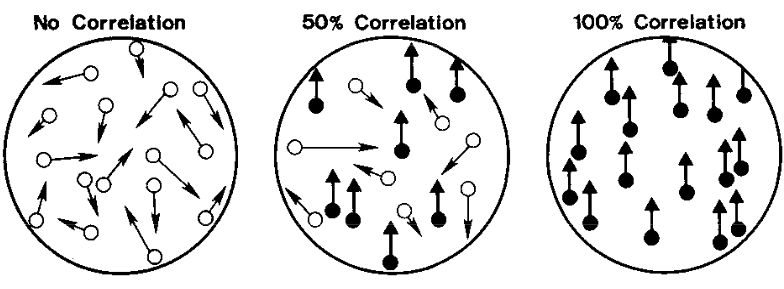
\includegraphics[width=0.75\linewidth]{figures/dots.PNG}
    \caption{A typical RDM task \citep{brittenAnalysisVisualMotion1992}}
    \label{fig:RDM}
\end{figure}

\section{Road Safety in Decision Neuroscience}
Road safety is multi factorial and can be approached from a variety of different directions. This includes through the application of DN techniques. \citet{pekkanenVariableDriftDiffusionModels2022} examined the timing of pedestrian crossing decisions using a variable-drift diffusion model. They showed that it could be used to effectively account for the time at which pedestrians chose to cross the road in a simulation of that situation. This is of particular note as it shows the capability of these models to capture the complexity of the decisions in the complex environment of road traffic. In \citet{zgonnikovShouldStayShould2024} researchers examined the 'gap acceptance' decision drivers make within the context of an evidence accumulation DDM. They showed a reliable method of modelling the behaviour of drivers in complex situations. Critically this involved some adaptations of the typical SAT paradigm to allow for the use of the oncoming cars 'time to arrival' as the measure of urgency.

\section{The Cognitive Neural Systems Lab}
This project takes place in the context of the work taking place in the Cognitive Neural Systems lab in UCD (The Kelly Lab) which has been examining the neural basis of decisions as aforementioned. Some of the work of the lab was examined as part of the literature review.

% Talk about why that can be applied to my situation
The models discussed in \citet{geuzebroekBalancingTrueFalse2023} were of particular note due to their focus on the decision making mechanisms that occur during a continuous monitoring task with intermittent detection of stimuli. This is a similar context to that which is the focus of this thesis; a driver must continuously monitor the situation in front of them and respond to a series of intermittent encounters with cyclists. Of the variety of models examined the best fit to the model was found to be the criterion adjustment model, a schematic of which can be seen in \ref{fig:Anna}. In this model the evidence accumulation was referenced to a zero criterion point that could be adjusted among task difficulty contexts. How these difficulty contexts can be understood in the scenario of a driving task will be the subject of further discussion.
Having a model which has been built to fit to this format of decisions allows us to parametrise behavioural data as it is gathered from the experiment. This will then allow us to examine the influence of a series of factors on the decisions that are made by subjects.
\begin{figure}[H]
    \centering
    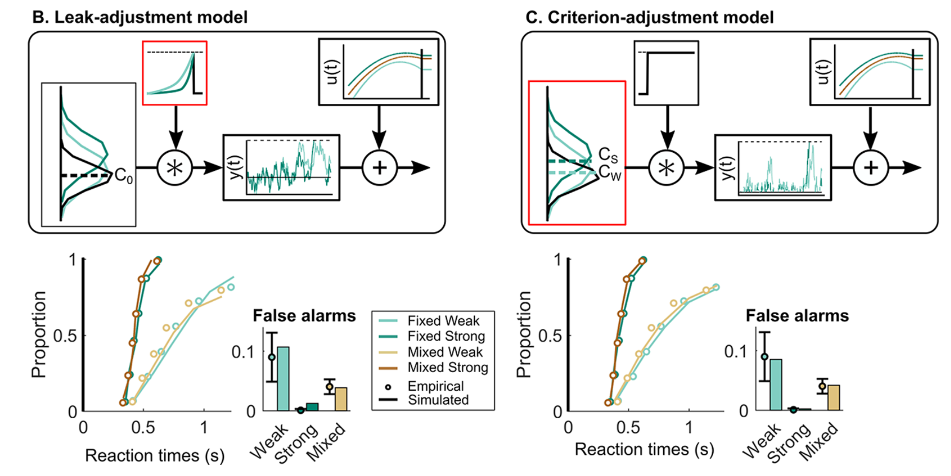
\includegraphics[width=0.75\linewidth]{figures/Anna.PNG}
    \caption{A figure from Geuzebroek et al comparing the fits of the B) leak-adjustment and C) criterion-adjustment models that were examined in the paper. While it is not clear which of the fits was better from this model what can be seen is that the models were successful in simulating data similar to the observed data \citep{geuzebroekBalancingTrueFalse2023}}
    \label{fig:Anna}
\end{figure}